\section{Introduction}
    \label{Section:Introduction}\needtodo{Talk about FHE?}
    With the advent of quantum computers cryptographic schemes based on problems not easily broken by quantum algorithms have risen in popularity. A group of such problems arise in the theory of lattices (Section \ref{Section:Lattice Theory}. A lattice is a discrete subspace of \(\mathbb{R}^n\). Some central, hard problems that naturally arise in lattice-based cryptography is to find the shortest vector in the lattice, the \emph{Shortest Vector Problem} (SVP), and finding the closest lattice-point to a vector in \(\mathbb{R}^n\), the \emph{Closest Vector Problem}. These two problems are closely related.\\
    % Input a figure of some lattice stuff
    \begin{figure}[h]
\center
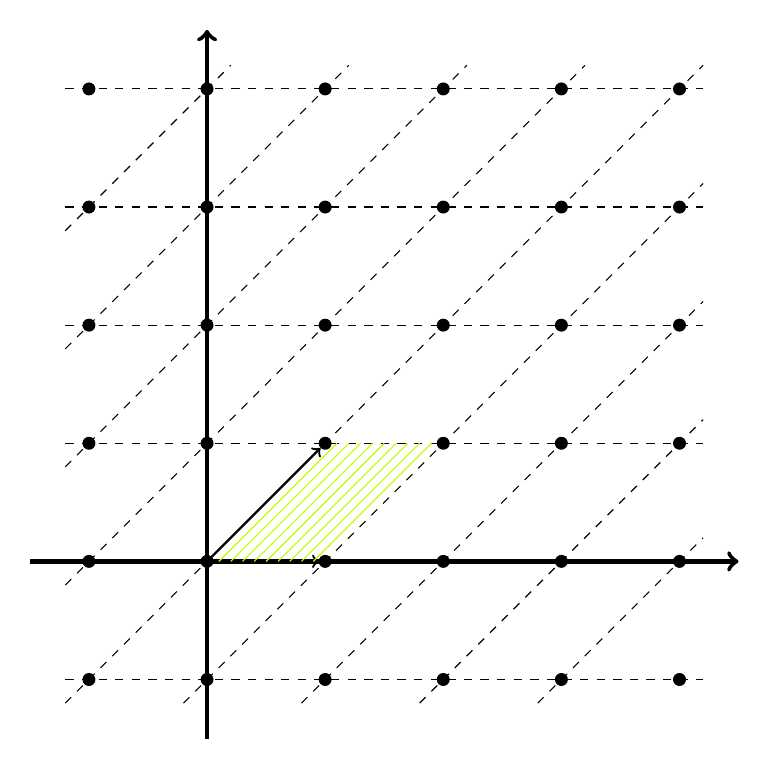
\begin{tikzpicture}[scale=1.5]

% AXES
\draw [ultra thick, ->] (-1.5, 0) -- (4.5, 0);
\draw [ultra thick, ->] (0, -1.5) -- (0, 4.5);

% BASIS VECTORS
\draw [thick, ->] (0, 0) -- (0.95, 0);
\draw [thick, ->] (0, 0) -- (0.96, 0.96);

% HORIZONTAL LINES
\draw [dashed, thin] (-1.2, 4) -- (4.2, 4);
\draw [dashed, thin] (-1.2, 3) -- (4.2, 3);
\draw [dashed, thin] (-1.2, 2) -- (4.2, 2);
\draw [dashed, thin] (-1.2, 1) -- (4.2, 1);
\draw [dashed, thin] (-1.2, -1) -- (4.2, -1);

% SKEW LINES
\draw [dashed] (-1.2, -0.2) -- (3.2, 4.2);
\draw [dashed] (-1.2, 0.8) -- (2.2, 4.2);
\draw [dashed] (-1.2, 1.8) -- (1.2, 4.2);
\draw [dashed] (-1.2, 2.8) -- (0.2, 4.2);
\draw [dashed] (-1.2, -1.2) -- (4.2, 4.2);
\draw [dashed] (-0.2, -1.2) -- (4.2, 3.2);
\draw [dashed] (0.8, -1.2) -- (4.2, 2.2);
\draw [dashed] (1.8, -1.2) -- (4.2, 1.2);
\draw [dashed] (2.8, -1.2) -- (4.2, 0.2);

% All intersection points
\draw[fill] (1,1) circle [radius=0.025];\draw[fill](-1,-1)circle [radius=0.050];\draw[fill](-1,0)circle [radius=0.050];\draw[fill](0,-1)circle [radius=0.050];\draw[fill](0,0)circle [radius=0.050];\draw[fill](1,-1)circle [radius=0.050];\draw[fill](1,0)circle [radius=0.050];\draw[fill](2,-1)circle [radius=0.050];\draw[fill](2,0)circle [radius=0.050];\draw[fill](3,-1)circle [radius=0.050];\draw[fill](3,0)circle [radius=0.050];\draw[fill](4,-1)circle [radius=0.050];\draw[fill](4,0)circle [radius=0.050];\draw[fill](-1,1)circle [radius=0.050];\draw[fill](-1,2)circle [radius=0.050];\draw[fill](0,1)circle [radius=0.050];\draw[fill](0,2)circle [radius=0.050];\draw[fill](1,1)circle [radius=0.050];\draw[fill](1,2)circle [radius=0.050];\draw[fill](2,1)circle [radius=0.050];\draw[fill](2,2)circle [radius=0.050];\draw[fill](3,1)circle [radius=0.050];\draw[fill](3,2)circle [radius=0.050];\draw[fill](4,1)circle [radius=0.050];\draw[fill](4,2)circle [radius=0.050];\draw[fill](-1,3)circle [radius=0.050];\draw[fill](-1,4)circle [radius=0.050];\draw[fill](0,3)circle [radius=0.050];\draw[fill](0,4)circle [radius=0.050];\draw[fill](1,3)circle [radius=0.050];\draw[fill](1,4)circle [radius=0.050];\draw[fill](2,3)circle [radius=0.050];\draw[fill](2,4)circle [radius=0.050];\draw[fill](3,3)circle [radius=0.050];\draw[fill](3,4)circle [radius=0.050];\draw[fill](4,3)circle [radius=0.050];\draw[fill](4,4)circle [radius=0.050];

% Fundamental paraleliped (?)

\draw[thin,color=lime] (0.1,0) -- (1.1, 1);
\draw[thin,color=lime] (0.2,0) -- (1.2, 1);
\draw[thin,color=lime] (0.3,0) -- (1.3, 1);
\draw[thin,color=lime] (0.4,0) -- (1.4, 1);
\draw[thin,color=lime] (0.5,0) -- (1.5, 1);
\draw[thin,color=lime] (0.6,0) -- (1.6, 1);
\draw[thin,color=lime] (0.7,0) -- (1.7, 1);
\draw[thin,color=lime] (0.8,0) -- (1.8, 1);
\draw[thin,color=lime] (0.9,0) -- (1.9, 1);



\end{tikzpicture}
\caption{Lattice with basis \(\mathfrak{B} = \{(1, 0), (1, 1)\}\). This lattice is isomorphic to the lattice with basis vectors \((1, 0)\) and \((-1, 1)\).}
\label{Figure:Lattice1}
\end{figure}
    
    Many efficient cryptosystems rely on \emph{ideal lattices}, which correspond to ideals in a certain ring\footnote{Namely \(\mathbb{Z}[X]/\langle f(x)\rangle\) for an irreducible \(f(x)\)}. Solving SVP in such lattices boils down to finding a 'short' generator for the ideal. We often assume that there exists a short generator, so that the search can succeed. There are two steps in finding such a generator for a principal ideal \cite{Recover Short Gen}.
    
    Firstly, find a generator for a principal ideal, which need not be short. This is called the \emph{principal ideal problem}. The results of \cite{Find Generator Classic} has show that this is possible to do classically in sub-exponential time, namely \(2^{N^{1/2 + O(1)}}\). Additionally, there exists a quanum polynomial time algorithm from \cite{Find Generator Quantum} which finds such a generator. Secondly, after a generator is found, transform it into a 'short' generator and thereby recover the secret key of the cryptosystems. A proof of the second part of the process was provided by \cite{Recover Short Gen}.
    
    The security of many modern lattice based cryptography schemes is based on the hardness of these problems. In particular, the security of the fully homomorphic scheme by Gentry \cite{Gentry} and schemes based on his methods, such as the one by Smart and Vercauteren\needtodo{Find source for this}, hinges on solving the SG-PIP problem. There is a classical reduction from SG-PIP to (LWE) by Peikert.\cite{Reduction PG-PIP LWE}\improvement{Read this source}. So finding a good solution to SG-PIP means that LWE is not hard, and assuming LWE is hard then these cryptosystems are secure in some sense.\improvement{Elaborate}\par
    
    The structure of this thesis is as follows: We start by introducing the general algebraic number theory required to understand the machinery used in various algorithms and problems. Then we present basic lattice theory and the hard problems used in cryptography associated with lattices. We discuss the relationship between hard problems and how they relate to security. Next, we present the algorithms for the first part of SG-PIP, discussing both the sub-exponential classic and quantum polynomial algorithm. From there we show how a found generator can be made 'short'. Any specific theory needed in either of these algorithms will be presented in that chapter.\newpage
\subsection{Glossary}
    To keep consistent notation, use the following notation my man
    \begin{itemize}
        \item \(K, L\) are a number fields, \(L\) extension of \(K\).
        
        \item \(R = \OO_K\): Ring of integers. Omit \(K\) if it is clear.
        
        \item \(\alpha\) are integral elements
        
        \item \(\Lambda\) is a lattice
        
        \item \(\mathcal{B}\) and \(\mathcal{B}^\vee\) are the basis and dual basis, respectively.
        
        \item \(\vec{b}\) and \(\vec{b}^\vee\) are basis vectors and dual basis vectors, respectively
        
        \item \(\fraka, \frakb\) are ideals
        
        \item \(\frakp, \frakq\) are prime ideals
        
        \item \(\calI\) is the group of fractional ideals, or just set of ideals
        
        \item Keep \(U\) to mean group of units of something, probably group of roots of unity.
        
        \item \(\sigma\) is the cannonical embedding. \(\tau\) is the coordiante embedding?
        
        \item \(d\) is a divisor.
        
    \end{itemize}